% Name: Git branching and merging
% Description: A feature branch that leaves main and merges back, a hotfix merged into main in the meantime and pulled into the feature, and a release tag.
% Tags: git, branching, merge, version control

\usetikzlibrary{arrows.meta}

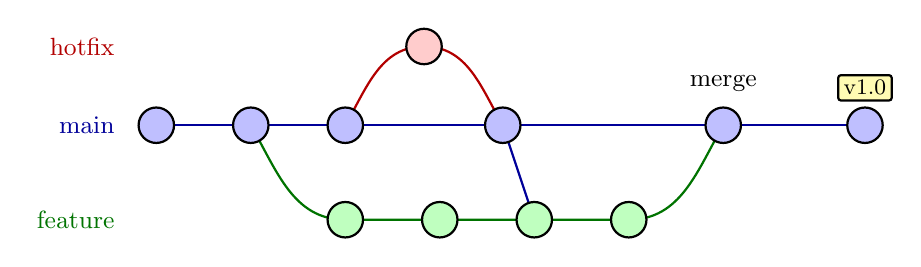
\begin{tikzpicture}[thick, every node/.style={font=\small},
    commit/.style={circle, draw, fill=#1, inner sep=0pt, minimum size=4.5mm}]
  % Lanes: main at y = 0, hotfix at y = 1, feature at y = -1.2. Edges point from parent to child.
  \node[anchor=east, blue!60!black] at (-0.4,0) {main};
  \node[anchor=east, red!70!black] at (-0.4,1) {hotfix};
  \node[anchor=east, green!45!black] at (-0.4,-1.2) {feature};
  \draw[blue!60!black] (0,0) -- (9,0);
  \draw[green!45!black] (1.2,0) to[out=-60, in=180] (2.4,-1.2) -- (6,-1.2) to[out=0, in=-120] (7.2,0);
  \draw[red!70!black] (2.4,0) to[out=60, in=180] (3.4,1) to[out=0, in=120] (4.4,0);
  % Main, with the hotfix in it, is merged into feature so the feature sees the fix before it merges back.
  \draw[blue!60!black] (4.4,0) -- (4.8,-1.2);
  \foreach \x in {0, 1.2, 2.4, 4.4, 7.2, 9} \node[commit=blue!25] at (\x,0) {};
  \foreach \x in {2.4, 3.6, 4.8, 6} \node[commit=green!25] at (\x,-1.2) {};
  \node[commit=red!20] at (3.4,1) {};
  \node[above=3mm] at (7.2,0) {merge};
  \node[draw, fill=yellow!30, rounded corners=1pt, inner sep=2pt, font=\footnotesize, above=3mm] at (9,0) {v1.0};
\end{tikzpicture}
